
\documentclass[12pt]{article}
\usepackage{fancyhdr}
\renewcommand{\familydefault}{\sfdefault}
\renewcommand*{\ttdefault}{\familydefault}
\usepackage[paperwidth=35cm,paperheight=50cm,left =1cm, top = 1cm, right =1cm, bottom = 1cm ,marginparwidth=0cm, includeheadfoot,headheight=66pt, headsep=0cm]{geometry}
\usepackage{pgfplots}
\pgfplotsset{width=5cm,compat=newest}
\usetikzlibrary{plotmarks}
\usepgfplotslibrary{dateplot}
\usepgfplotslibrary{units}
\tikzset{every picture/.append style={font=\normalsize}} % size graph font
\usetikzlibrary{arrows, positioning, calc}

\tikzstyle{chart}=[
legend label/.style={font={\Large},anchor=west,align=left},
legend box/.style={rectangle, draw, minimum size=5pt},
axis/.style={black,semithick,->},
axis label/.style={anchor=east,font={\tiny}}]

\definecolor{customcolor}{HTML}{1d5893}
\begin{document}
\begin{minipage}{0.96\linewidth}
\flushleft
\begin{tikzpicture}
\pgfplotscreateplotcyclelist{defaultCycle}{%
ybar,%ybar legend,
fill=customcolor,draw=black,opacity=1,thin,solid,mark=no,mark options=solid,\\%
}


    
\begin{axis}
[
%    xbar, <--- comment this line 
    cycle list name=defaultCycle,
    width=0.8\linewidth,
    height=0.15\textheight,
    use units,
    scale only axis,
    symbolic x coords={JMA,ERM,ADMIN},
    xtick=data,
    nodes near coords,
    yticklabel style={/pgf/number format/fixed},,
    ytick pos=left,
    axis y line*=left,
    xtick pos=bottom,
    axis x line*=bottom,
    legend style={draw=none,at={(0,1.03)},anchor=south west},
    legend columns=-1,
    xtick align=center,
    ytick align=center,
    xtick distance=0.1,
    ytick distance=,
    x tick label style ={font=\normalsize,text width=0.3cm,anchor=north,rotate=0,align=center},
    y tick label style ={font=\normalsize,text width=2cm,anchor=east,rotate=0,align=right},
    scaled y ticks=false,
    bar width=35pt,
    ymajorgrids,
    ylabel=\textbf{Number of Hours Worked},
    xlabel=\textbf{Task Name},
    title=\textbf{Craig's Work Week Breakdown},
    ,
    ]

        \addplot  + table [x={x},y={y},meta index=2,col sep=comma] {
        x, y, z
        JMA, 15, 0
        ERM, 10, 0
        ADMIN, 10, 0
        };

\end{axis}
\end{tikzpicture}
\end{minipage}


\end{document}

\newpage



    
\begin{axis}
[
%    xbar, <--- comment this line 
    cycle list name=defaultCycle,
    width=0.8\linewidth,
    height=0.15\textheight,
    use units,
    scale only axis,
    symbolic x coords={unplanned,POM25,POM26},
    xtick=data,
    nodes near coords,
    yticklabel style={/pgf/number format/fixed},,
    ytick pos=left,
    axis y line*=left,
    xtick pos=bottom,
    axis x line*=bottom,
    legend style={draw=none,at={(0,1.03)},anchor=south west},
    legend columns=-1,
    xtick align=center,
    ytick align=center,
    xtick distance=0.1,
    ytick distance=,
    x tick label style ={font=\normalsize,text width=0.3cm,anchor=north,rotate=0,align=center},
    y tick label style ={font=\normalsize,text width=2cm,anchor=east,rotate=0,align=right},
    scaled y ticks=false,
    bar width=35pt,
    ymajorgrids,
    ylabel=\textbf{Number of Hours Worked},
    xlabel=\textbf{Task Name},
    title=\textbf{Craig's Work Week Breakdown},
    ,
    ]

        \addplot  + table [x={x},y={y},meta index=2,col sep=semicolon] {
        x; y; z
        unplanned; 5; 0
        POM25; 25; 0
        POM26; 25; 0
        };

\end{axis}
\end{tikzpicture}
\end{minipage}

\newpage



    
% \begin{axis}
% [
% %    xbar, <--- comment this line 
%     cycle list name=defaultCycle,
%     width=0.8\linewidth,
%     height=0.15\textheight,
%     use units,
%     scale only axis,
%     symbolic x coords={Admin,24BES,24Spend plan},
%     xtick=data,
%     nodes near coords,
%     yticklabel style={/pgf/number format/fixed},,
%     ytick pos=left,
%     axis y line*=left,
%     xtick pos=bottom,
%     axis x line*=bottom,
%     legend style={draw=none,at={(0,1.03)},anchor=south west},
%     legend columns=-1,
%     xtick align=center,
%     ytick align=center,
%     xtick distance=0.1,
%     ytick distance=,
%     x tick label style ={font=\normalsize,text width=0.3cm,anchor=north,rotate=0,align=center},
%     y tick label style ={font=\normalsize,text width=2cm,anchor=east,rotate=0,align=right},
%     scaled y ticks=false,
%     bar width=35pt,
%     ymajorgrids,
%     ylabel=\textbf{Number of Hours Worked},
%     xlabel=\textbf{Task Name},
%     title=\textbf{Craig's Work Week Breakdown},
%     ,
%     ]

%         \addplot  + table [x={x},y={y},meta index=2,col sep=semicolon] {
%         x; y; z
%         Admin; 15; 0
%         24BES; 15; 0
%         24Spend plan; 17; 0
%         };

% \end{axis}
% \end{tikzpicture}
% \end{minipage}

% \newpage



\end{document}